\subsection{Context Reweights a Fixed Token Row}

The previous sections varied targets and inspected feature competition within
low-error preferences. Here we keep the token row fixed and vary the prompt,
asking how context changes the profile term \(h^\top d_i\) while the token-row
coefficients remain fixed.

\paragraph{Context reweighting.}
Holding the target token fixed isolates this context-dependent factor. In
\Cref{fig:same-token-polysemy}, Qwen3.5-2B reweights
\texttt{bug}, \texttt{ring}, and \texttt{bridge} toward context-appropriate
feature families. Each displayed centered-token account has relative
reconstruction error below \(0.05\), using the same \(\rho\) convention as the
fidelity tables. For example, the \texttt{bug} row shifts from mosquito- and bee-like
features to defect-, crash-, and debug-like features; \texttt{bridge} shifts
from river/crossing features to networking features. Additional prompt-level
views are in Appendix~\ref{app:additional-qwen-display-examples}.
Because fitted token-row coefficients are fixed after training the readout SAE,
the displayed change isolates the hidden-state profile.

\begin{figure}[t]
    \centering
    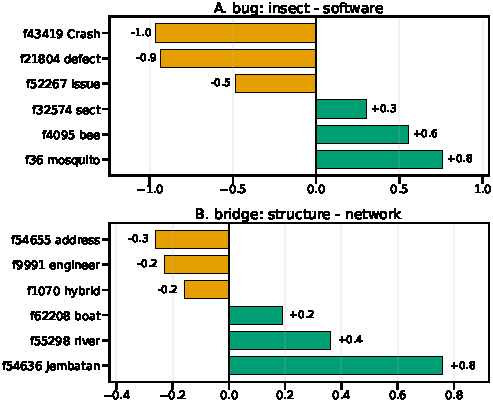
\includegraphics[width=\columnwidth]{figures/proto_token_lens/qwen2b_32x_domain_features_main3/qwen2b_32x_polysemy_delta_row_onecol.pdf}
    \caption{\textbf{Same selected token, different prompt contexts.}
    Each panel keeps the output token fixed and subtracts the second prompt
    context from the first for $h^\top(w_t-\mu)$. Teal/orange bars are larger in
    the first/second context; the axis is change in signed contribution.}
    \label{fig:same-token-polysemy}
\end{figure}
